

\documentclass{article}
\usepackage{amsmath}
\usepackage{graphicx}
\usepackage[margin=0.8in]{geometry}
\usepackage{titling}

\renewcommand\maketitlehooka{\null\mbox{}\vfill}
\renewcommand\maketitlehookd{\vfill\null}
\renewcommand{\figurename}{Supplementary Figure}

\title{Mapping short reads, faithfully: supplementary figures}

\author{%
Eduard Valera Zorita,
Ruggero Cortini,
Guillaume J. Filion}

\begin{document}

\begin{titlingpage}
\maketitle
\end{titlingpage}

\begin{figure}
\begin{center}
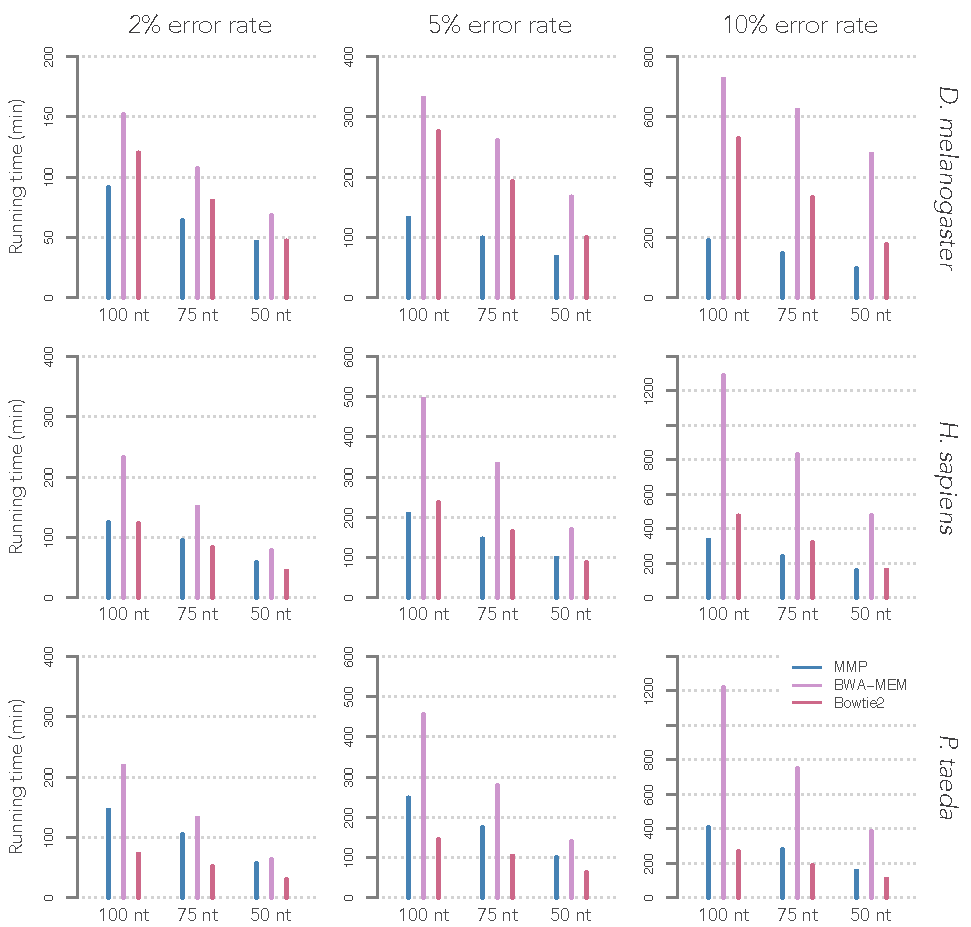
\includegraphics[scale=.53]{timem_supp.pdf}
\end{center}
\caption{Resource usage at 2, 5 and 10\% error rate. The representations
are as in Figure~8 (the memory footprint does not depend on the error rate
of the sequencing process).}
\end{figure}

\begin{figure}
\begin{center}
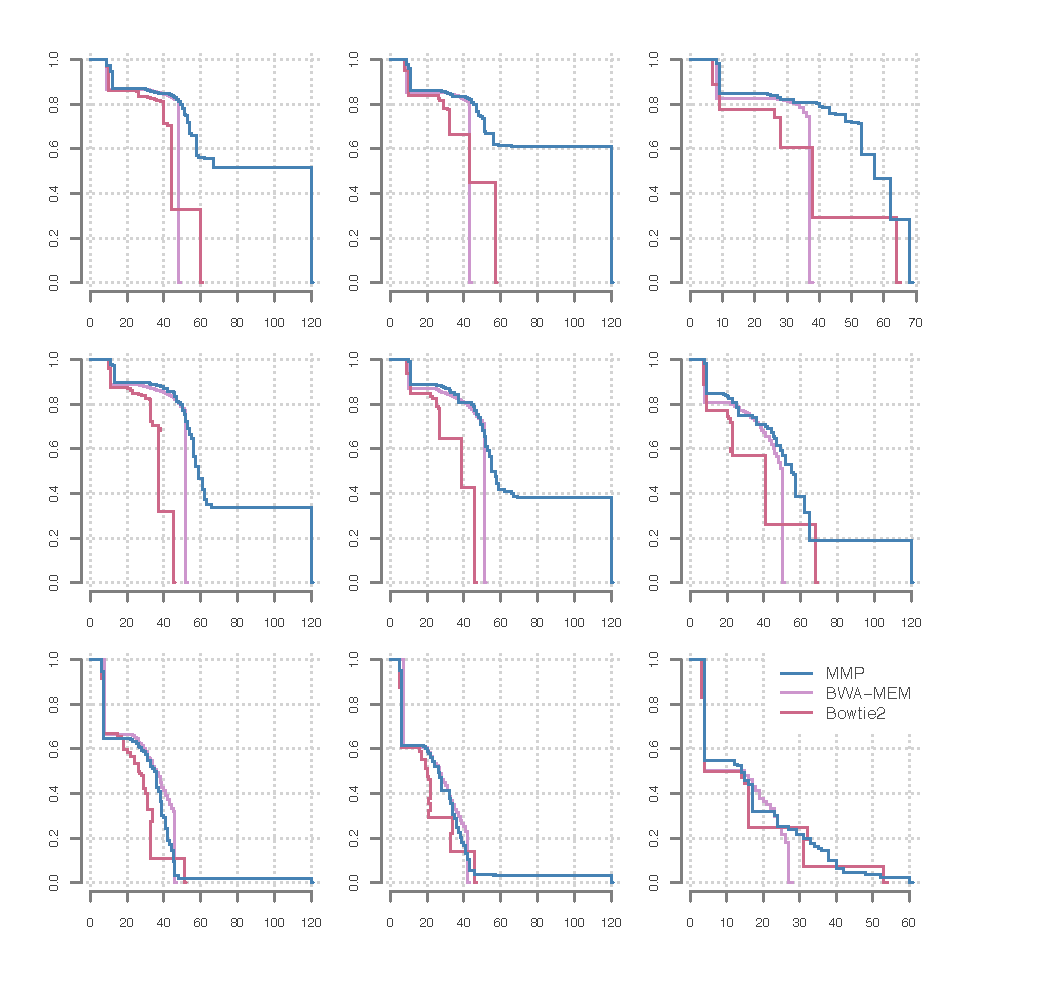
\includegraphics[scale=.54]{accQ2_fig.pdf}
\end{center}
\caption{Mapping accuracy with 2\% error rate. The representations are
as in Figure~7.}
\end{figure}

\begin{figure}
\begin{center}
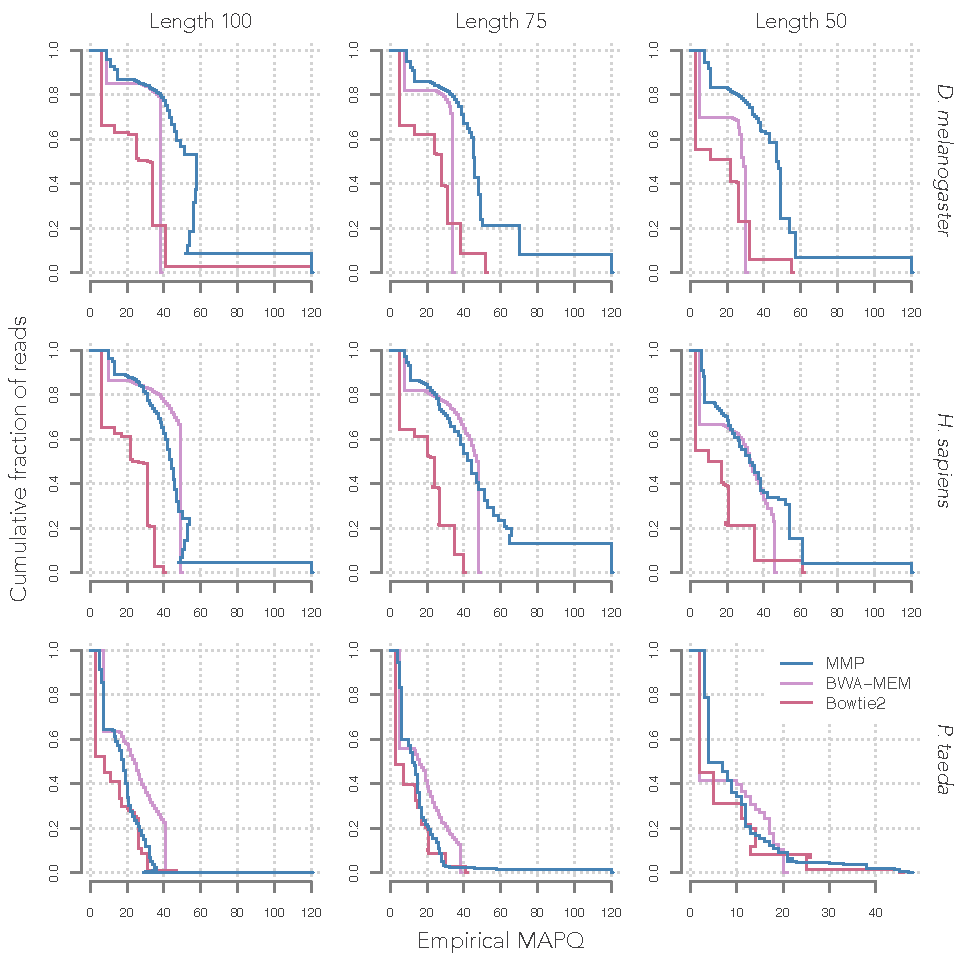
\includegraphics[scale=.54]{accQ5_fig.pdf}
\end{center}
\caption{Mapping accuracy with 5\% error rate. The representations are
as in Figure~7.}
\end{figure}

\begin{figure}
\begin{center}
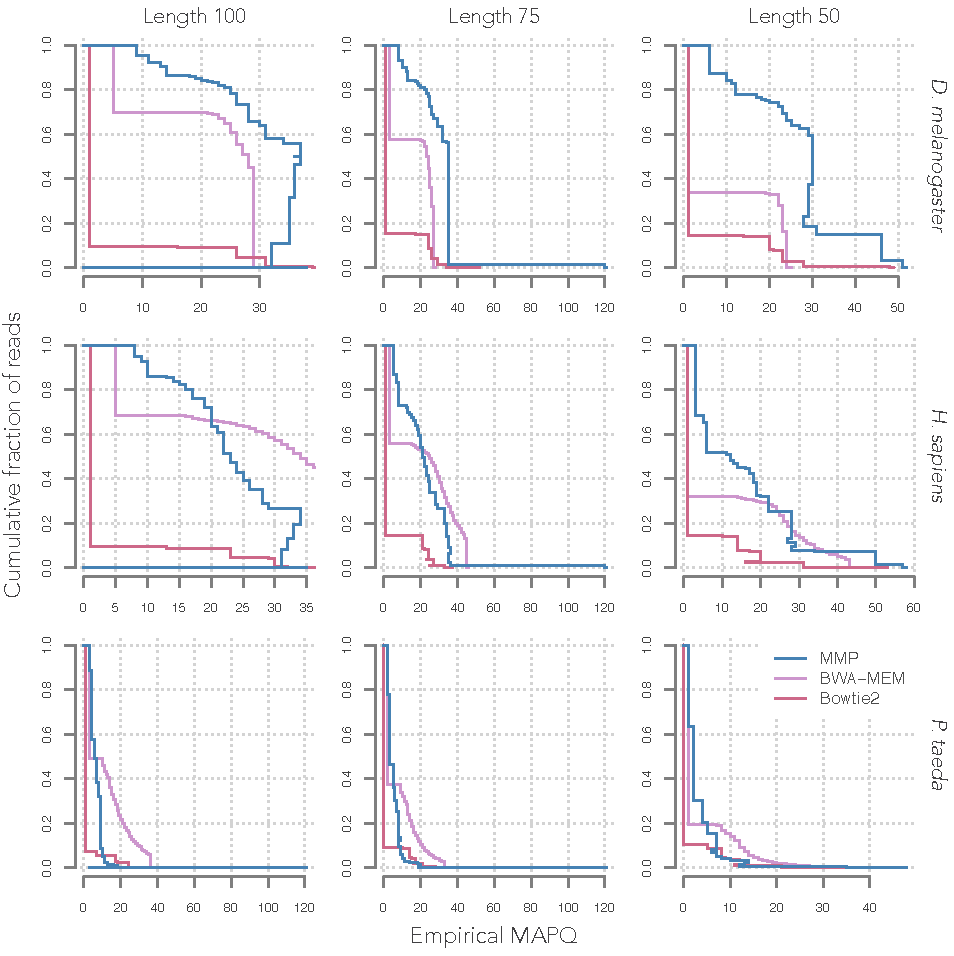
\includegraphics[scale=.54]{accQ10_fig.pdf}
\end{center}
\caption{Mapping accuracy with 10\% error rate. The representations are
as in Figure~7.}
\end{figure}

\clearpage

\begin{figure*}
\begin{center}
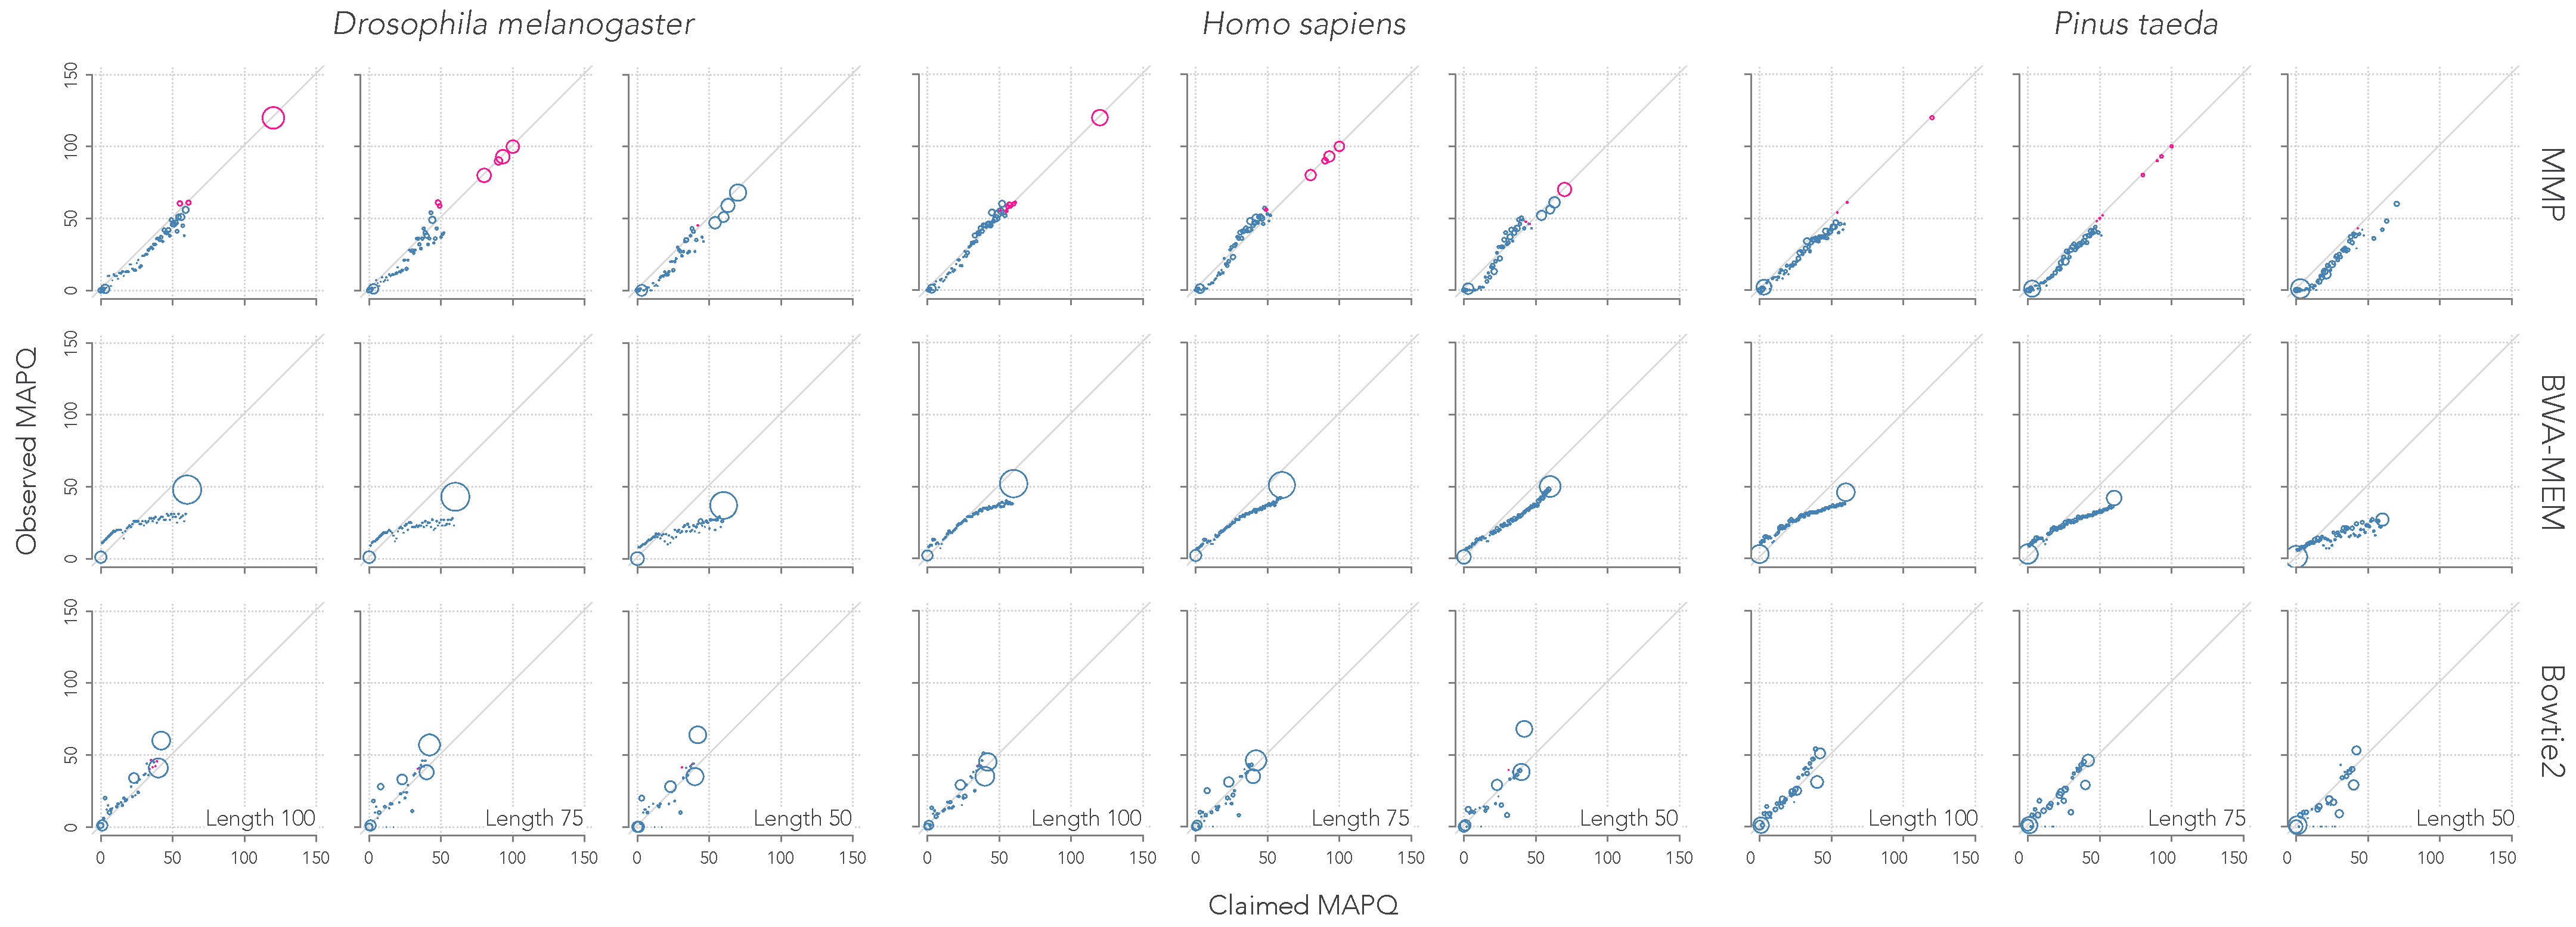
\includegraphics[scale=.24]{faith_Q2.pdf}
\end{center}
\caption{Faithfulness with 2\% error rate. The representations are
the same as in Figure~6.}
\end{figure*}

\begin{figure*}
\begin{center}
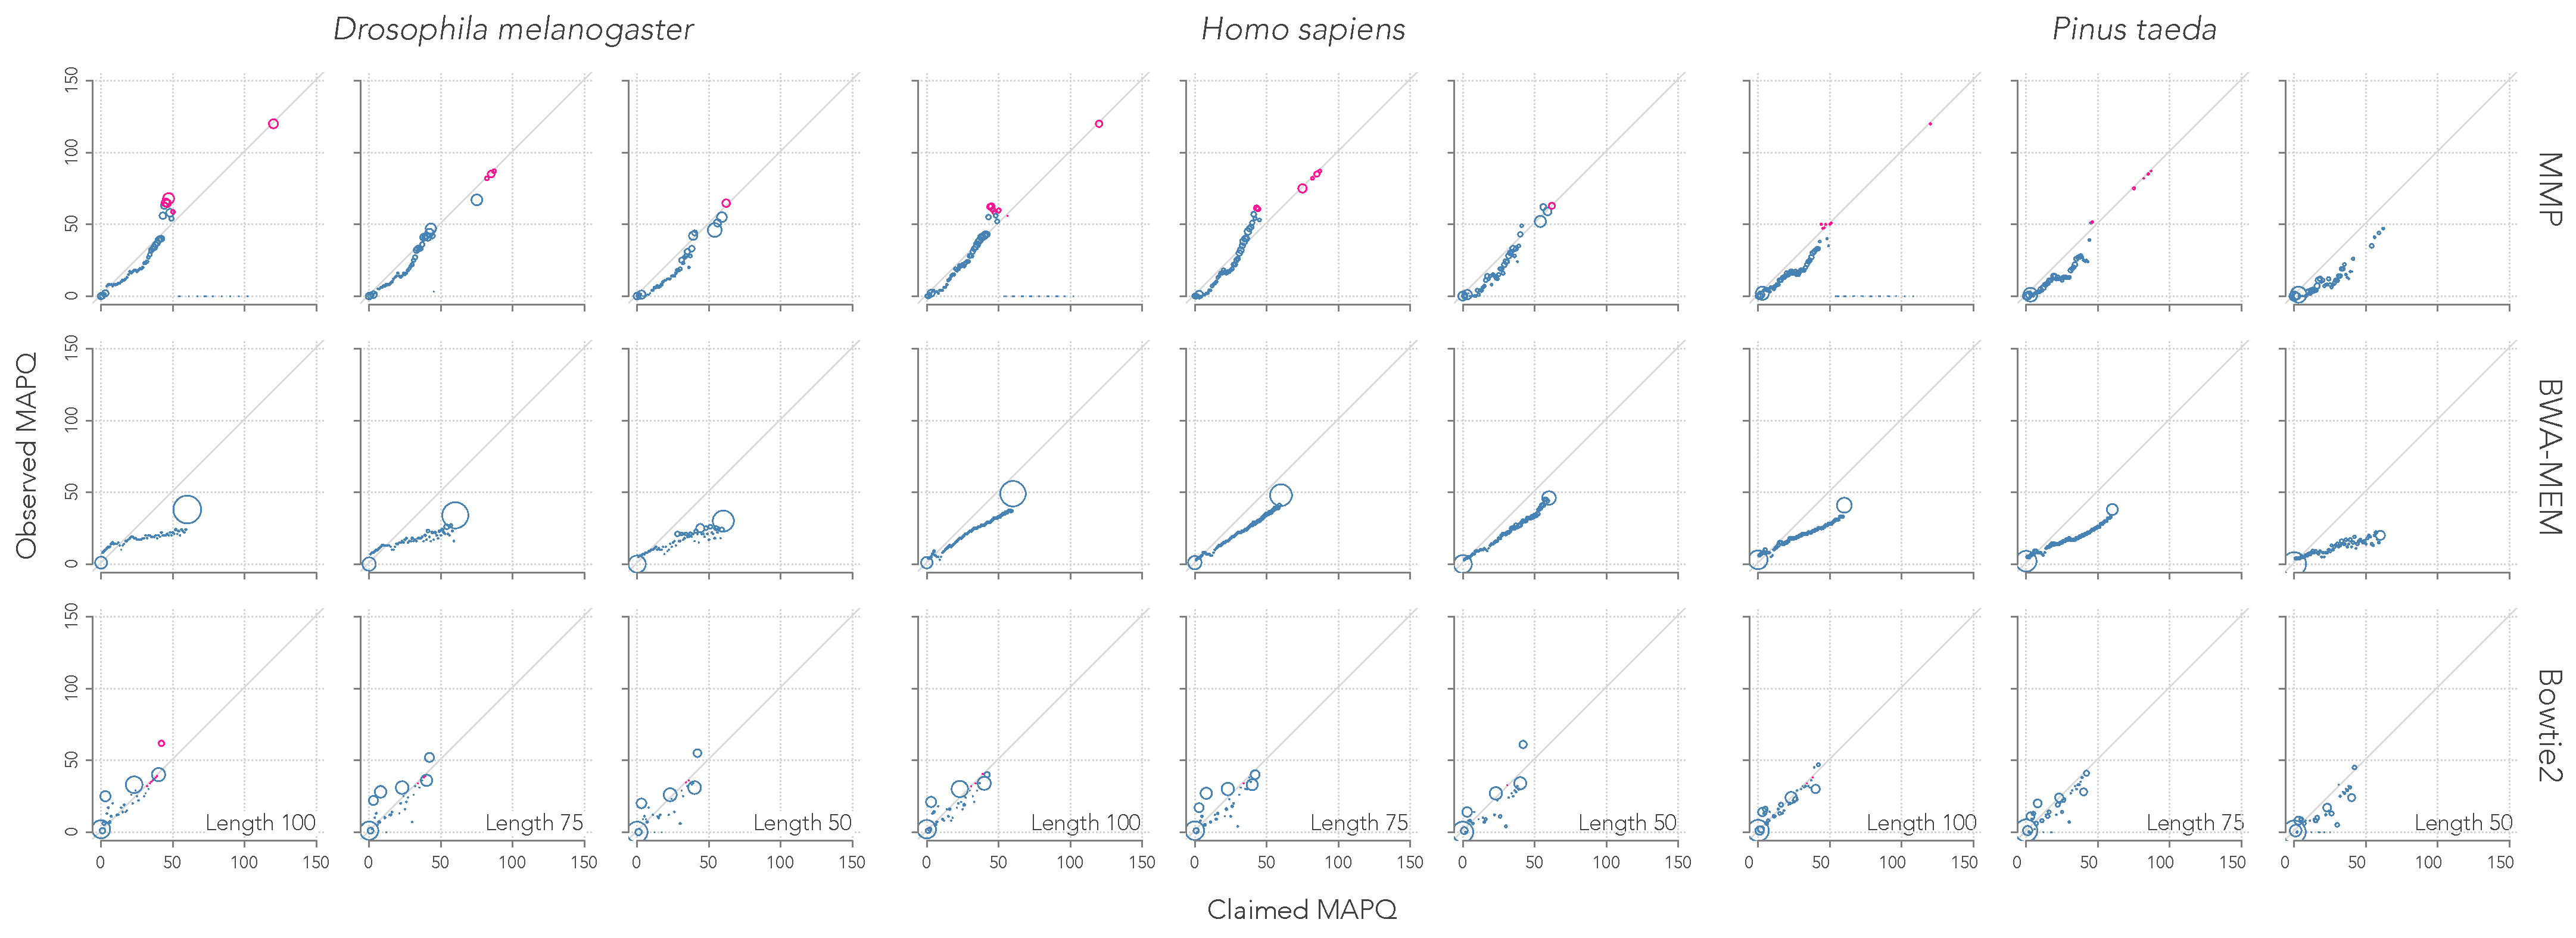
\includegraphics[scale=.24]{faith_Q5.pdf}
\end{center}
\caption{Faithfulness with 5\% error rate. The representations are
the same as in Figure~6.}
\end{figure*}

\begin{figure*}
\begin{center}
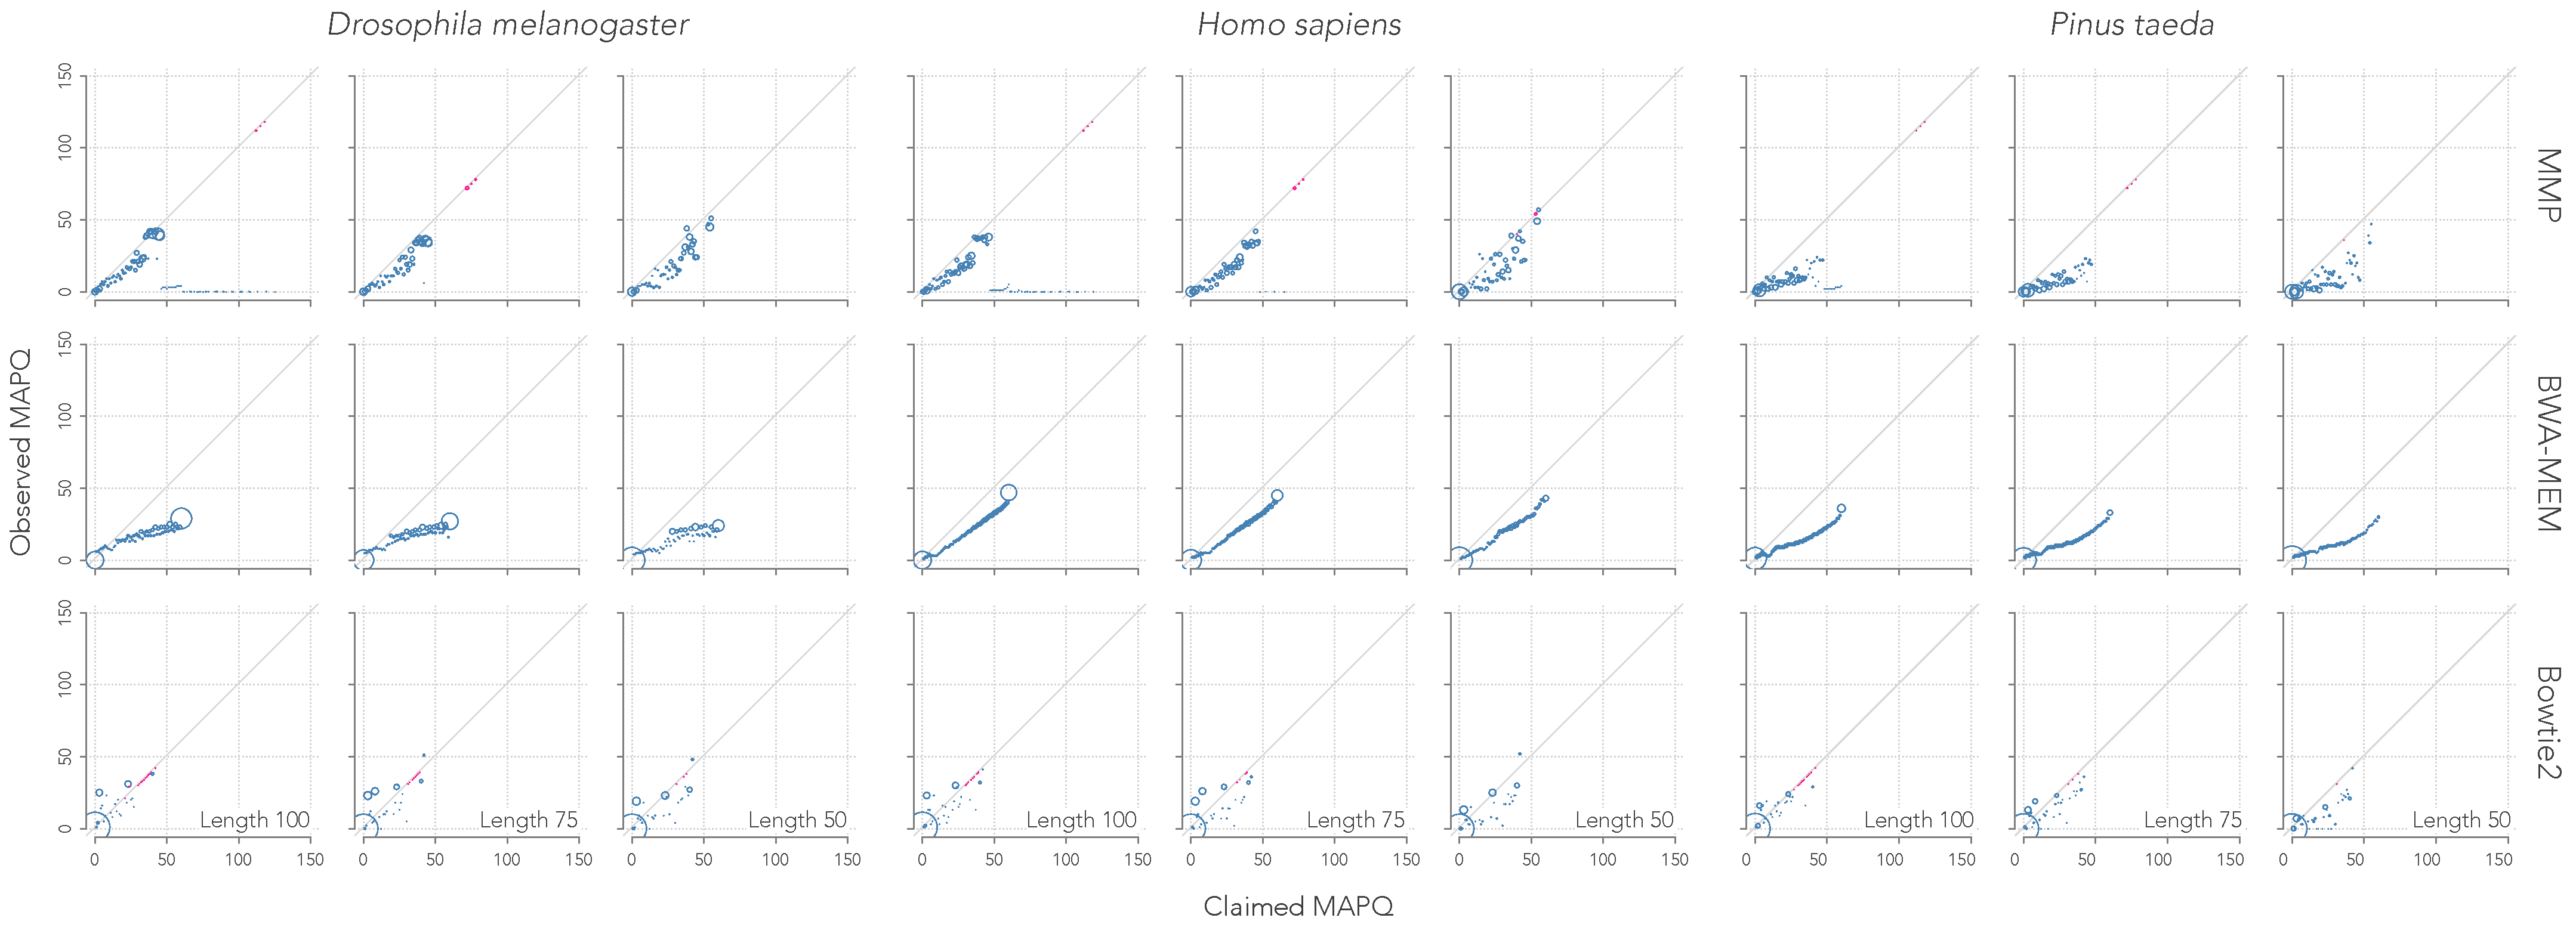
\includegraphics[scale=.24]{faith_Q10.pdf}
\end{center}
\caption{Faithfulness with 10\% error rate. The representations are
the same as in Figure~6.}
\end{figure*}
\end{document}
